%!TeX root=../tese.tex
%("dica" para o editor de texto: este arquivo é parte de um documento maior)
% para saber mais: https://tex.stackexchange.com/q/78101/183146

% Apague as duas linhas abaixo (elas servem apenas para gerar um
% aviso no arquivo PDF quando não há nenhum dado a imprimir) e
% insira aqui o conteúdo dos apêndices do seu trabalho (ou deixe
% este arquivo vazio)

\providecommand\aviso[1]{
  \clearpage
  \null
  \vfill
  \begin{hyphenrules}{nohyphenation}
    \centering\bfseries\Large
    #1\par
  \end{hyphenrules}
  \vfill
  \clearpage
}

\providecommand\avisoFolhasDeRosto{
  \aviso{
    {\huge Você precisa editar os arquivos no diretório ``\texttt{conteudo}''!}
    \par\bigskip\bigskip\bigskip\bigskip
    Para gerar a capa e demais páginas preliminares no formato correto,
    modifique os arquivos ``\texttt{conteudo/paginas-preliminares.tex}'' e
    ``\texttt{conteudo/metadados.tex}'', usando como base os arquivos
    correspondentes no diretório ``\texttt{conteudo-exemplo}''.
  }
}

\providecommand\avisoCapitulos{
  \aviso{
    Insira o conteúdo dos capítulos do seu trabalho no arquivo
    ``\texttt{capitulos.tex}'' do diretório ``\texttt{conteudo}''.
  }
}

\providecommand\avisoApendices{
  \aviso{
    Insira o conteúdo dos apêndices do seu trabalho no arquivo
    ``\texttt{apendices.tex}'' do diretório ``\texttt{conteudo}''.
  }
}

\providecommand\avisoAnexos{
  \aviso{
    Insira o conteúdo dos anexos do seu trabalho no arquivo
    ``\texttt{anexos.tex}'' do diretório ``\texttt{conteudo}''.
  }
}

\providecommand\avisoArtigo{
  \aviso{
    Insira o conteúdo do artigo no arquivo ``\texttt{corpo-artigo.tex}''
    do diretório ``\texttt{conteudo}''. Não se esqueça de consultar
    o exemplo no diretório ``\texttt{conteudo-exemplo}'' para a
    definição do título, autoria etc.
  }
}

\providecommand\avisoApresentacao{
  \begin{frame}{Insira o conteúdo!}
  \aviso{
    Insira o conteúdo da apresentação no arquivo ``\texttt{corpo-apresentacao.tex}''
    do diretório ``\texttt{conteudo}''. Não se esqueça de consultar
    o exemplo no diretório ``\texttt{conteudo-exemplo}'' para a
    definição do título, autoria, estrutura etc.
  }
  \end{frame}
}

\providecommand\avisoPoster{
  \aviso{
    Insira o conteúdo do poster no arquivo ``\texttt{corpo-poster.tex}''
    do diretório ``\texttt{conteudo}''. Não se esqueça de consultar
    o exemplo no diretório ``\texttt{conteudo-exemplo}'' para a
    definição do título, autoria, estrutura etc.
  }
}

\chapter{GSoC Propoal}\label{appendex1}
\label{ap:gsoc}

\definecolor{darkgreen}{RGB}{0, 133, 117}
\definecolor{yelloworange}{HTML}{FAA21A}

\begin{center}
\Huge \bf
\vspace{0.5cm}
\end{center}
\vspace*{\fill}
{
     \centering
     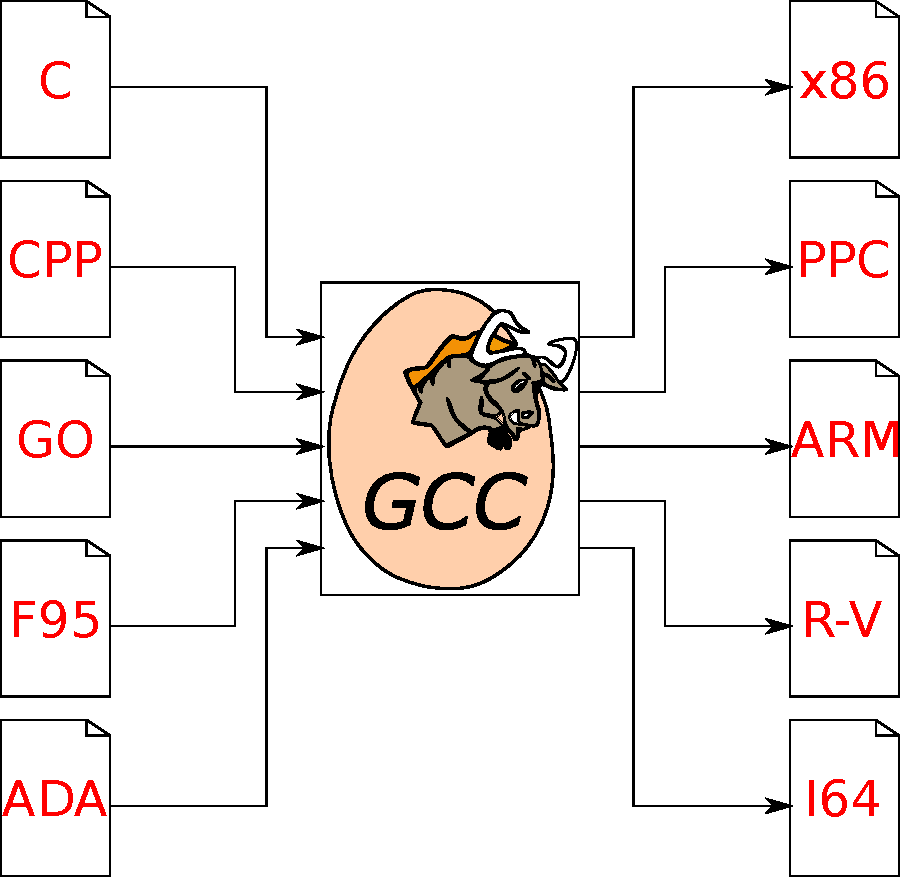
\includegraphics[scale=0.7]{logo.pdf}
    \par
}
\vspace*{\fill}
\normalsize{
\noindent\textcolor{darkgreen}{Giuliano Belinassi} \\
Timezone: GMT$-$3:00 \\
University of São Paulo -- Brazil \\
IRC: giulianob in \#gcc \\
Email: \href{mailto:giuliano.belinassi@usp.br}{\texttt{giuliano.belinassi@usp.br}} \\
Github: \url{https://github.com/giulianobelinassi/} \\
Date: April 1, 2019
}
\newpage

\begin{section}{About Me}
    Computer Science Bachelor (University of São Paulo), 
    currently pursuing a Masters Degree in Computer Science at the same
    institution. I've always been fascinated by topics such as
    High-Performance Computing and Code Optimization, having worked with
    a parallel implementation of a Boundary Elements Method software in GPU.
    I am currently conducting research on compiler parallelization and,
    therefore, a GSoC internship working with the GNU
    Compiler Collection (GCC) on a related topic is an excellent opportunity
    for me to become more involved with the Free Software community.

    \textbf{Skills}: Strong knowledge in C, Concurrency, Shared Memory Parallelism, command line utilities (grep, sed\dots) and other typical programming tools.
\end{section}

\begin{subsection}{Contributions to GCC}

I've submitted some patches, mainly adding inline optimizations to
trigonometric functions. This kind of patch requires exaustive testing to guarantee
that the optimization does not yield severely incorrect results. This work
resulted in a blog post\footnote{\url{https://flusp.ime.usp.br/gcc/2019/03/26/making-gcc-optimize-some-trigonometric-functions/}} 
about the patch \textit{Optimize sin(arctan(x))}.
I did this blog post both to register how to add this kind of optimization
and also to encourage newcomers to contribute to GCC.

\begin{table}[!htbp]
\centering
\begin{tabular}{|l|l|}
\hline
Name                                                                                      & Status   \\ \hline
    \href{https://patchwork.ozlabs.org/patch/981596/}{Optimize $\sin (\arctan (x))$}      & \color{darkgreen}{\texttt{Accepted}} \\ \hline
    \href{https://patchwork.ozlabs.org/patch/1003988/}{Optimize $\sinh (\text{arctanh} (x))$}   & \color{darkgreen}{\texttt{Accepted}} \\ \hline
    \href{https://patchwork.ozlabs.org/patch/961362/}{Fix typo 'exapnded'}                & \color{darkgreen}{\texttt{Accepted}} \\ \hline
    \href{https://en.wikibooks.org/wiki/LaTeX/Hyperlinks}{Split 'opt and gen' variable}   & \color{yelloworange}{\texttt{Working on}} \\ \hline
    \href{https://patchwork.ozlabs.org/patch/1023211/}{Update $\sin (\arctan (x))$ test}  & \color{yelloworange}{\texttt{Waiting Stage1}} \\ \hline
    \href{https://patchwork.ozlabs.org/patch/1046302/}{Fix PR89437}                           & Wilco Dijkstra version accepted \\ \hline
\end{tabular}
    \caption{}
\end{table}

\end{subsection}

\begin{section}{Parallelization Project}
While looking for topics in the compiler field that touched subjects that I
am interested for my masters thesis, I found a
parallelization project proposed in GSoC 2018. With this in mind, I started a
discussion in the mailing list to understand what that project is about,
which was parallelizing GCC internals to be able to compile big files
faster\footnote{\url{https://gcc.gnu.org/ml/gcc/2018-11/msg00073.html}}.
As can be seen in the discussion, I started to work on this subject way before
the list of GSoC accepted organizations was made public.

As stated in PR84402\footnote{\url{https://gcc.gnu.org/bugzilla/show\_bug.cgi?id=84402}},
there is a parallelism bottleneck in GCC concerning huge files (with hundreds of
thousands of lines of code). In the course of the discussion,
Bin Cheng\footnote{\url{https://gcc.gnu.org/ml/gcc/2018-12/msg00079.html}}
reported that
he is affected by this issue, stating that parallelizing the
compiler may solve his problem. These discussions demonstrate the
community interest in this project.

\begin{subsection}{Current Status}
In PR84402, Martin Liška posted a graphic showing the existence of a
parallelism bottleneck in GCC compilation due to huge files such as
\texttt{gimple-match.c} in a 128-cores machine that \texttt{make -j128} alone could not alleviate. He also posted an amazing patch to
GNU Make to collect the data and a script to plot the graphic, which I used
to reproduce the same behaviour in a 64-cores machine that is available at
my university.

Unfortunately, I found this approach not easy to replicate, as
it requires compiling and installing a custom version of Make and generates
gigabytes of data which require parsing by a script that often crashes, as
it struggles to generate a very large SVG. With this in mind, I created a set of
tools\footnote{\url{https://github.com/giulianobelinassi/gcc-timer-analysis}}
using a completely distinct approach, which generates less data, is more stable, and
plots better graphics, such as the one in Figure \ref{fig:analysis}.

I also explored the GCC codebase in order to find the performance bottleneck for
such huge files. I compiled GCC with the
\texttt{--disable-checking} and \texttt{-O2} flags, which
give a more performant (but less reliable) compiler and used this version to compile
\texttt{gimple-match.c} (the largest file in GCC). In this context, I found that the method
\texttt{finalize\_compilation\_unit()} of
class \texttt{symbol\_table} takes around $50s$ of the compilation time, with the
\texttt{expand\_all\_functions}
routine taking most of it. Therefore, this routine is a strong candidate for parallelization.

Currently, my strategy to parallelize \texttt{expand\_all\_functions()} is to
perform the \texttt{GIMPLE} processing step in parallel, as suggested
by Richard Biener\footnote{\url{https://gcc.gnu.org/ml/gcc/2019-03/msg00249.html}}: each
function may be independently processed by the many passes of
\texttt{GIMPLE}.  There is also a pipelined alternative: a distinct
thread is responsible for a given \texttt{GIMPLE} pass and each
function is fed sequentially to each of them. This allows many
functions to be processed simultaneously, each by a different pass.

Furthermore, I am also studying the theoretical background behind \texttt{GIMPLE}
and \texttt{cgraphs}. I have read the \texttt{GIMPLE}
documentation\footnote{\url{https://gcc.gnu.org/onlinedocs/gccint/}} and
I am looking at how \texttt{cgraph} works internally, both in theory and within
GCC.

\end{subsection}

\begin{subsection}{Planned Tasks}

I plan to use the GSoC time to develop the following topics:

\begin{itemize}
 \item{Week [1, 7] -- May 6 to June 21:} \\
Refactor \texttt{cgraph\_node::expand()} and
\texttt{expand\_all\_functions()}, splitting \texttt{IPA},
\texttt{GIMPLE} and \texttt{RTL} passes, and some documentation about
the global states of the \texttt{GIMPLE} passes.
 \item{Week 8 -- June 24 to 28:} \textbf{First Evaluation} \\
Deliver a patch with the refactored version of both functions mentioned above,
plus the partial documentation with regard to \texttt{GIMPLE}.
 \item{Week [9, 11] -- July 1 to 19:} \\
Continue documentating and refactoring the \texttt{GIMPLE} passes, and
prototype a parallelization of \texttt{expand\_all\_functions()}.
 \item{Week 12 --- July 22 to 26:} \textbf{Second Evaluation} \\
Attend to Debconf 19 (Curitiba, Brazil). Please let me know
if someone else from GCC will attend. \\
Deliver a
working non-optimized parallel version of \texttt{expand\_all\_functions()}
with the point of being correct in a multi-threaded environment.
\item{Week [13, 15] --- July 29 to August 16:} \\
Iteractively improve the current implementation.
\item{Week 16 - August 19:} \textbf{Final evaluation}\\
Optimize the current implementation, so that there is a speedup over
the sequential version when compiling \texttt{gimple-match.c} and reducing the
total compilation time in \texttt{GCC} compilation without bootstrap.
\end{itemize}

\begin{figure}[ht]
 \centering
 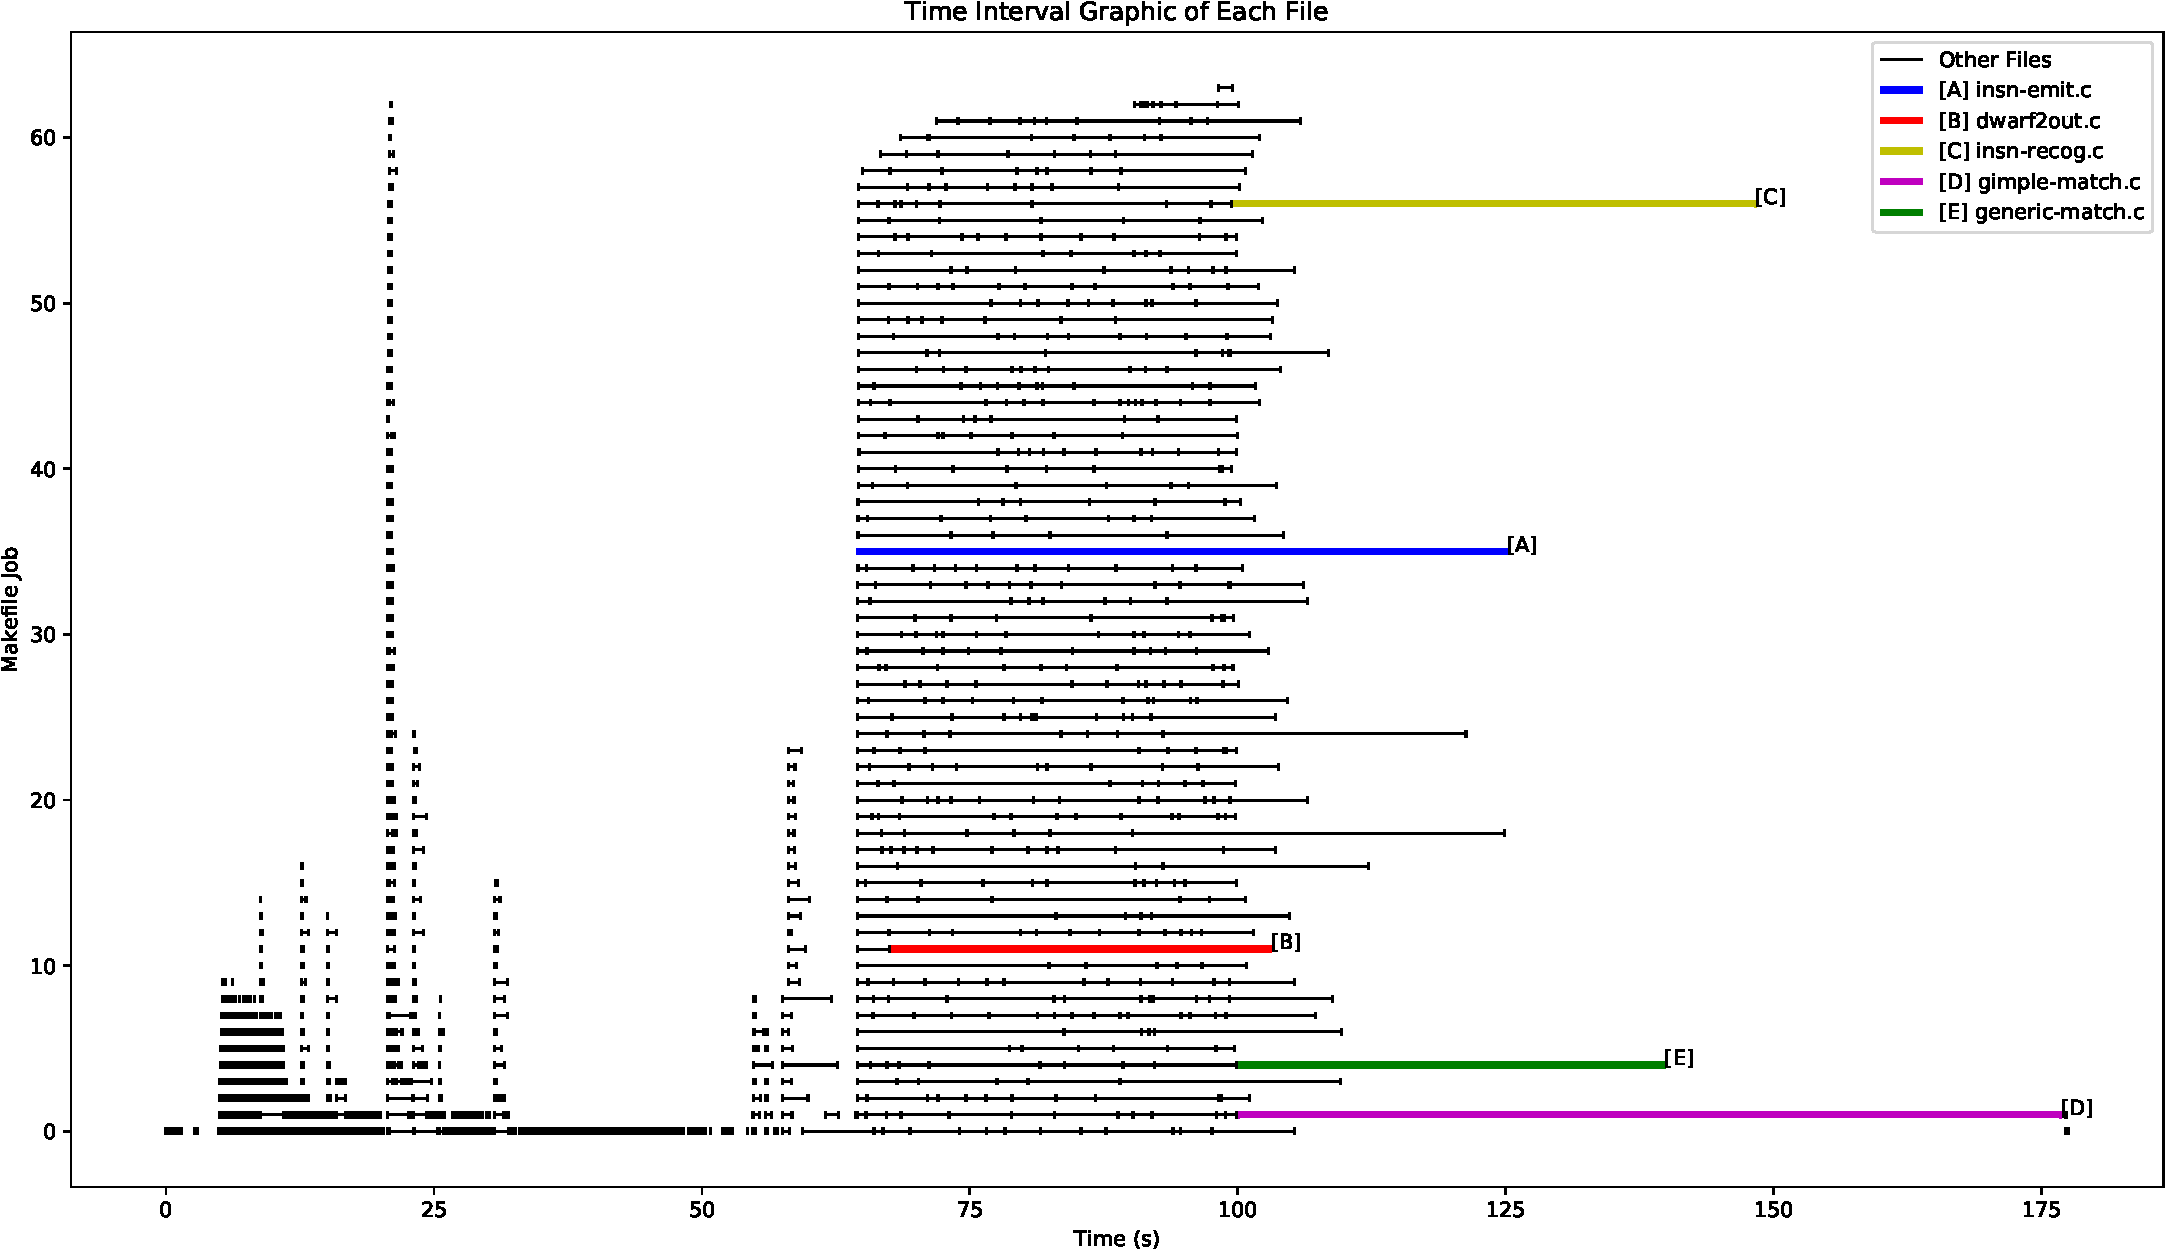
\includegraphics[scale=0.6, angle=-90]{out-crop.pdf}
 \caption{Elapsed time analysis in GCC compilation for a 64 cores machine, No bootstrap}
 \label{fig:analysis}
\end{figure}

\end{subsection}

\end{section}


%% Template baseado no do Prof. Arnaldo Mandel
%% Veja https://www.ime.usp.br/~am/414/listas/index.html

%\documentclass[12pt]{article}

%% Escrevendo em português:

%\usepackage[brazilian]{babel}
%\usepackage[utf8]{inputenc}
%%\usepackage{textcomp}
%\usepackage[T1]{fontenc}
%\usepackage{lmodern}
%%----------------------------
%
%\setlength{\topmargin}{-.5in}
%\setlength{\textheight}{9in}
%\setlength{\textwidth}{6.3in}
%\setlength{\oddsidemargin}{-.125in}
%\setlength{\evensidemargin}{-.125in}
%
%\usepackage[usestackEOL]{stackengine}
%\usepackage{xspace}
%\usepackage{pifont}
%\usepackage{amsmath}
%\usepackage{amsfonts}
%\usepackage[dvipsnames]{xcolor}
%\usepackage{fancybox}
%\usepackage{amsthm}
%\usepackage{listings}
%\usepackage{hyperref}
%\usepackage{todonotes}
%
%\usepackage{MnSymbol,wasysym}
%\usepackage{marvosym}
%
%\pagestyle{empty}
%
%\definecolor{darkgreen}{RGB}{0, 133, 117}
%\definecolor{yelloworange}{HTML}{FAA21A}
%
%\newcommand{\N}{{\tt I\kern-.2em N \relax}}      % N        |N
%\def\pule{\vspace{0.2cm}}
%\def\pulao{\vspace{0.5cm}}
%\def\pulaozao{\vspace{1cm}}
%\def\ni{\noindent}
%
%\newcommand{\Si}{\ensuremath{\Sigma}\xspace}
%\newcommand{\Sis}{\ensuremath{\Sigma^*}\xspace}
%\newcommand{\Ga}{\ensuremath{\Gamma}\xspace}
%\newcommand{\Gas}{\ensuremath{\Gamma^*}\xspace}
%\newcommand{\serio}{\ding{98}\xspace}
%\newcommand{\LP}{L\&P\xspace}
%\newcommand{\conj}[2]{\ensuremath{\{#1\,|\;#2\}}}
%\DeclareMathOperator{\Ima}{Im}
%\newcommand{\ssq}{\ensuremath{\subseteq}\xspace}
%\newcommand{\union}{\mathop{\bigcup}\displaylimits}
%\newcommand{\Rfield}[1]{\ensuremath{\mathbb{R}^{#1}}\xspace}
%\newcommand{\del}{\ensuremath{\text{d}}\xspace}
%\newcommand{\expct}[1]{\ensuremath{\langle {#1} \rangle}\xspace}
%
%\begin{document}
%
%\newtheorem{theorem}{Teorema}%[section]
%\newtheorem{corollary}{Corolário}[theorem]
%\newtheorem{lemma}[theorem]{Lema}

\chapter{Automatic Detection of Parallel Compilation Viability}
\vspace*{\fill}
{
     \centering
     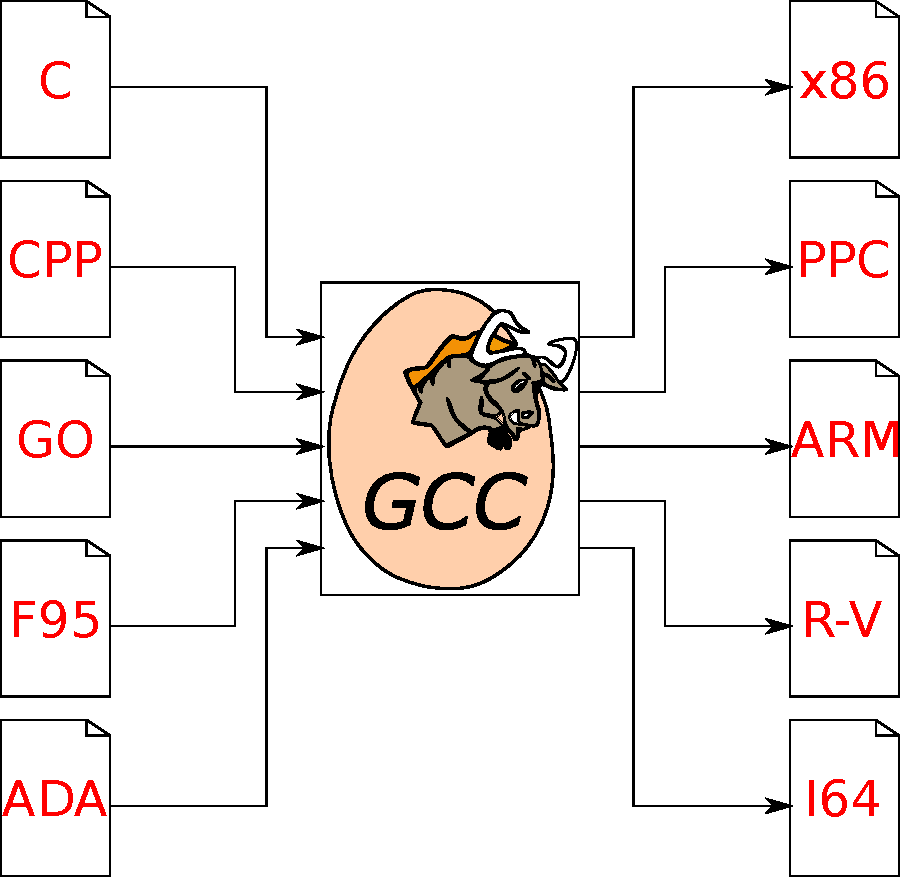
\includegraphics[scale=1.0]{logo.pdf}
    \par
}
\vspace*{\fill}
\normalsize{
\noindent\textcolor{darkgreen}{Giuliano Belinassi} \\
Timezone: GMT$-$3:00 \\
University of São Paulo -- Brazil \\
IRC: giulianob in \#gcc \\
Email: \href{mailto:giuliano.belinassi@usp.br}{\texttt{giuliano.belinassi@usp.br}} \\
Github: \url{https://github.com/giulianobelinassi/} \\
Date: \today
}
\newpage

\begin{section}{About Me}
    Computer Science Bachelor (University of São Paulo),
    currently pursuing a Masters Degree in Computer Science at the same
    institution. I've always been fascinated by topics such as
    High-Performance Computing and Code Optimization, having worked with
    a parallel implementation of a Boundary Elements Method software in GPU.
    I am currently conducting research on compiler parallelization and
    developing the \href{https://gcc.gnu.org/wiki/ParallelGcc}{ParallelGcc} project,
    having already presented it in \href{https://www.youtube.com/watch?v=jd6R3IK\_\_1Q}{GNU Cauldron 2019}.

    \textbf{Skills}: Strong knowledge in C, Concurrency, Shared Memory
    Parallelism, Multithreaded Debugging and other typical programming tools.
\end{section}

\begin{section}{Brief Introduction}

In \href{https://gcc.gnu.org/wiki/ParallelGcc}{ParallelGcc}, we showed that parallelizing the Intra Procedural optimizations
improves speed when compiling huge files by a factor of 1.8x in a 4 cores
    machine, and also showed that this takes 75\% of compilation time.

In this project we plan to use the LTO infrastructure to improve
compilation performance in the non-LTO case, with a tradeoff of generating
a binary as good as if LTO is disabled. Here, we will automatically detect
when a single file will benefit from parallelism, and procceed with the
compilation in parallel if so.

\begin{section}{Use of LTO}

The Link Time Optimization (LTO) is a compilation technique that allows the
compiler to analyse the program as a whole, instead of analysing and compiling
one file at time. Therefore, LTO is able to collect more information about
the program and generate a better optimization plan. LTO is divided in three
parts:

\begin{itemize}
    \item \emph{LGEN (Local Generation)}: Each file is translated to GIMPLE. This
        stage runs sequentially in each file and, therefore, in parallel in
        the project compilation.

    \item \emph{WPA (Whole Program Analysis)}: Run the Inter Procedural Analysis (IPA) in the
        entire program. This state runs serially in the project.

    \item \emph{LTRANS (Local Transformation)}: Execute all Intra Procedural Optimizations in
        each partition. This stage runs in parallel.
\end{itemize}

Since WPA can bottleneck the compilation because it runs serially in the entire
project, LTO was designed to produce faster binaries, not to produce binaries
fast.

Here, the proposed use of LTO to address this problem is to run the IPA
for each Translation Unit (TU), instead in the Whole Program, and automatically
detect when to partition the TU into multiple LTRANS to improve compilation performance.

The advantage of this approach is: by partitioning big files into multiple
partitions, we can improve the compilation performance by exposing these
partitions to the Jobserver. Therefore, it can improve CPU utilization in
manycore machines.  Generated code quality should be unaffected by this
procedure, which means that it should run as fast as when LTO is disabled.



\begin{itemize}

    \item It can generate binaries as good as when LTO is disabled.
    \item It is faster, as we can partition big files into multiple partitions
    and compile these partitions in parallel.
    \item It can interact with GNU Make Jobserver, improving CPU utilization.

\end{itemize}

\end{section}

\begin{section}{Planned Tasks}

I plan to use the GSoC time to develop the following topics:

\begin{itemize}
 \item{Week [1, 4] -- May 4 to May 27:} \\
  Update \texttt{cc1}, \texttt{cc1plus}, \texttt{f771}, \ldots, to partition
  the Compilation Unit (CU) after IPA analysis directly into multiple LTRANS
  partitions, instead of generating a temporary GIMPLE file, and to accept a
  additional parameter \texttt{-fsplit-outputs=<tempfile>}, in which the
  generated ASM filenames will be written to.

  There are two possible cases in which I could work on:
  \begin{enumerate}
    \item \textit{Fork}: After the CU is partitioned into multiple LTRANS, then
    \texttt{cc1} will fork and compile these partitions, each of them
    generating a ASM file, and write the generated asm name into
    \texttt{<tempfile>}.  Note that if the number of partitions is one, then
    this part is not necessary.

    \item \textit{Stream LTRANS IR}: After CU is partitionated into multiple
    LTRANS, then \texttt{cc1} will write these partitions into disk so that LTO
    can read these files and proceed as a standard LTO operation in order to
    generate a partially linked object file.
  \end{enumerate}

  1. Has the advantage of having less overhead than 2., as there is less IO operations,
  however it may be hard to implement as the assembler file may be already
  opened before forking, so caution is necessary to make sure that there are a
  1 - 1 relationship between assembler file and the compilation process. 2.
  on the other hand can easily interact with the GNU jobserver.

 \item{Week [5, 8] -- June 1 to June 26:} \\
  Update the \texttt{gcc} driver to take each file in \texttt{<tempfile>}, then
  assemble and partially link them together. Here, an important optimization is
  to use a named pipe in \texttt{<tempfile>} to avoid having to wait every
  partition to end its compilation before assembling the files.

 \item{Week 9 -- June 29 to July 3:} \textbf{First Evaluation} \\
  Deliver a non-optimized version of the project. Some programs ought to be
  compiled correctly, but probably there will be a huge overhead because so far
  there is no way of interacting with GNU Jobserver.

 \item{Week [10, 12] -- July 6 to July 24:} \\
  Work on GNU Make Jobserver integration. A way of doing this is to adapt
  the LTO WPA $\rightarrow$ LTRANS way of interacting with Jobserver. Another
  way is to make the forked \texttt{cc1} consume Jobserver tokens until the
  compilation finishes, then return the token when done.

 \item{Week 13 -- July 27 to 31:} \textbf{Second Evaluation} \\
  Deliver a more optimized version of the project. Here we should filter files
  that would compile fast from files that would require partitioning, and
  interact with GNU Jobserver. Therefore we should see some speedup.

\item{Week [14, 16] -- August 3 to 21:} \\
  Develop adequate tests coverage and address unexpected issues
  so that this feature can be merged to trunk for the next GCC
  release.

\item{Week 17: August 24 to 31} \textbf{Final evaluation}\\
  Deliver the final product as a series of patches for trunk.


\end{itemize}
\end{section}

\end{section}
\end{document}

\avisoApendices

% Os apêndices podem ser inseridos diretamente aqui ou "puxados" de outros
% arquivos.
% Em alguns (raros) casos, pode ser interessante usar \include ao
% invés de \input: https://tex.stackexchange.com/a/32058/183146

%\input{conteudo/...}
%\par
